\documentclass[french,english]{article}
\usepackage[T1]{fontenc}
\usepackage[utf8]{inputenc}
\usepackage{fixltx2e}
\usepackage{graphicx}
% \usepackage{listings}
\usepackage{babel}
\usepackage{color}
\usepackage{colortbl}
\usepackage{listings}
\usepackage{pxfonts}

\lstset{
    language=Caml,
    basicstyle=\ttfamily,
    keywordstyle=\color[rgb]{0.5,0,0}\bfseries,
    commentstyle=\color[rgb]{0.133,0.545,0.133},
    showstringspaces=false,
    frame=tb,
    columns=fullflexible,
    morekeywords={undefined}
}

\definecolor{Gray}{gray}{0.85}

\begin{document}
  \section{Brouillon}
  \subsection{Analyse d'un bloc de base}
  Le programme parcourt les blocs de base linéairement en mettant à jour la liste de prédicats.

  Nous définissons d'abord une fonction d'invalidation d'une variable dans la liste de prédicats, qui consiste à
  supprimer tous les prédicats qui utilisent cette variable.

  \begin{lstlisting}[mathescape]
    invalidate var p =
        {predicate $\in$ p $|$ var $\notin$ predicate}
  \end{lstlisting}

  Il s'agit maintenant de définir l'effet de la lecture de chaque instruction sur la liste de prédicats.
  Exemple sur un premier cas trivial :

  \begin{lstlisting}
    t [NOP] p =
        p (* rien ne change *)
  \end{lstlisting}

  La fonction de traduction \texttt{t} opère sur une instruction (ici \texttt{NOP}) et la liste de prédicats \texttt{p}.

  Regardons maintenant comment est traitée l'instruction d'assignation d'une variable à une autre variable (\texttt{SET}) :

  \begin{lstlisting}
    t [SET d a] p =
        (d = a) @ (invalidate d p)
  \end{lstlisting}

  Un nouveau prédicat \texttt{d = a} est généré après qu'on ait invalidé \texttt{d},
  c'est-à-dire qu'on ait supprimé tous les prédicats qui contiennent t.
  De même pour l'instruction \texttt{SETI} qui assigne une constante à une variable.

  \begin{lstlisting}
    t [SETI d cst] p =
        (d = a) @ (invalidate d p)

    t [CMP d a b] p =
        (d = a ~ b) @ (invalidate d p)
    \end{lstlisting}

    Cet opérateur $\sim$ bien spécifique aux langages d'assembleur sert à se souvenir que
    \texttt{d} contient des informations sur la comparaison entre \texttt{a} et \texttt{b}.

    Pour la suite nous allons avoir besoin de la fonction \texttt{update} qui sert à remplacer
    toutes les occurences d'une variable \texttt{var} par l'expression \texttt{expr} dans la liste de prédicats \texttt{p} :

  \begin{lstlisting}[mathescape]
    update var expr p =
        {predicate[expr / var] $|$ predicate $\in$ p}
  \end{lstlisting}

  où la syntaxe \texttt{predicate[expr / var]} dénote ici le prédicat où le terme \texttt{var} est remplacé par l'expression \texttt{expr}.

  \begin{lstlisting}[mathescape]
    t [ADD d a b] p =
        if (d = a) then (* d <- d+b *)
            (update d (d - b) p)
        else if (d = b) (* d <- a+d *)
            (update d (d + a) p)
        else
            (d = a + b) @ (invalidate d p)

    t [SUB d a b] p =
        if (d = a) then
            if (d = b) then (* d <- d-d *)
                (update d 0 p)
            else (* d <- d-b *)
                (update d (d+b) p)
        else
            if (d = b) then (* d <- a-d *)
                (update d (a-d) p)
            else (* d <- a-b *)
                (d = a - b) @ (invalidate d p)

    t [MUL d a b] p =
        if (d = a) then
            if (d = b) then (* d <- d*d *)
                (* impossible de remplacer d par $\sqrt{d}$, on invalide *)
                (0 <= d) @ (invalidate d p)
            else (* d <- d*b *)
                (* on rajoute un predicat pour indiquer que d est
                   divisible par b *)
                (d % b = 0) @ (update d (d/b) p)
        else
            if (d = b) then (* d <- a*d *)
                (d % a = 0) @ (update d (d/a) p)
            else (* d <- a*b *)
                (d = a * b) @ (invalidate d p)

    t [DIV d a b] p =
        if (d = a) then
            if (d = b) then (* d <- d/d *)
                (d = 1) @ (invalidate d p)
            else (* d <- d/b *)
                (* impossible de remplacer d par (d*b),
                   on a perdu de l'information ! *)
                (invalidate d p)
        else
            if (d = b) then (* d <- a/d *)
                (invalidate d p)
            else (* d <- a/b *)
                (d = a / b) @ (invalidate d p)
  \end{lstlisting}

  Pour illustrer le problème de l'instruction DIV, prenons le cas où l'on a \texttt{\{t1 = 7, t2 = 3\}} et une instruction \texttt{[DIV t1 t1 t2]}.\\
  En remplaçant \texttt{t1} par \texttt{t1 * t2}, on obtiendrait \texttt{\{(t1 * t2 = 7), (t2 = 3)\}}, c'est-à-dire \texttt{(t1 * 3 = 7)}, ce qui est impossible puisqu'on travaille sur des entiers !

  \begin{lstlisting}
    t [MOD d a b] p =
        if (d = a or d = b)
            (invalidate d p)
        else
            (d = a % b) @ (invalidate d p)
  \end{lstlisting}

  Nous utiliserons dans la suite une fonction \texttt{eval} qui cherche la valeur \textbf{constante} pour une variable.
  La fonction eval parcourt donc la liste des prédicats à la recherche de prédicats du type \texttt{(var = 2)} permettant
  d'identifier la valeur de \texttt{var}.

  \begin{lstlisting}
    t [ASR d a b] p =
        let b_val = eval b in
        if b_val is undefined then
            (invalidate d p)
        else
            let factor = 2 ** b_val in
            if (d = a) then (* d <- d>>b *)
                (update d (d / factor) p)
            else (* d <- a>>b *)
                (d = a / factor) @ (invalidate d p)

    t [NEG d a] =
        if (a = d) (* d <- -d *)
            (update d (-d) p)
        else (* d <- -a *)
            (d = -a) @ (invalidate d p)
  \end{lstlisting}



  \subsection{Brouillon1}
  \begin{figure}
    \begin{center}
      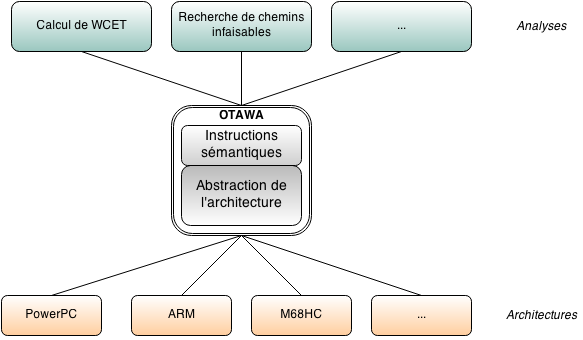
\includegraphics[scale=0.5]{pictures/otawa_abstraction_architecture.png}
    \end{center}
    \caption{OTAWA permet aux analyses de s'abstraire de l'architecture}
  \end{figure}
  \begin{figure}
    \begin{tabular}{|l|l|} \hline
      \textbf{Instruction} & \textbf{Sémantique}\\ \hline \hline
      \texttt{NOP} & (rien)\\ \hline
      \texttt{BRANCH} & \\
      \texttt{TRAP} & Indicateurs du flot du programme\\
      \texttt{CONT} & \\ \hline
      \texttt{IF cond sr jump} & si la condition \texttt{cond} sur le registre \texttt{sr} est vraie, continuer,\\
      & sinon sauter \texttt{jump} instructions\\ \hline
      \texttt{LOAD reg addr type} & reg $\leftarrow$ \texttt{MEM\textsubscript{type}} \\ \hline
      \texttt{STORE reg addr type} & \texttt{MEM\textsubscript{type}} $\leftarrow$ \texttt{reg}\\ \hline
      \texttt{SCRATCH d} & \texttt{d $\leftarrow$ $\top$} \textit{(invalidation)}\\ \hline
      \texttt{SET d a} & \texttt{d $\leftarrow$ a}\\ \hline
      \texttt{SETI d cst} & \texttt{d $\leftarrow$ cst}\\ \hline
      \rowcolor{Gray} \texttt{SETP d cst} & \texttt{page(d) $\leftarrow$ cst}\\ \hline
      \texttt{CMP d a b} & \texttt{d $\leftarrow$ a $\sim$ b}\\ \hline
      \rowcolor{Gray} \texttt{CMPU d a b} & \texttt{d $\leftarrow$ a $\sim$\textsubscript{unsigned} b}\\ \hline
      \texttt{ADD d a b} & \texttt{d $\leftarrow$ a $+$ b}\\ \hline
      \texttt{SUB d a b} & \texttt{d $\leftarrow$ a $-$ b}\\ \hline
      \rowcolor{Gray} \texttt{SHL d a b} & \texttt{d $\leftarrow$ unsigned(a) <{<} b}\\ \hline
      \rowcolor{Gray} \texttt{SHR d a b} & \texttt{d $\leftarrow$ unsigned(a) >{>} b}\\ \hline
      \texttt{ASR d a b} & \texttt{d $\leftarrow$ a >{>} b}\\ \hline
      \texttt{NEG d a} & \texttt{d $\leftarrow$ $-$a}\\ \hline
      \rowcolor{Gray} \texttt{NOT d a} & \texttt{d $\leftarrow$ $\neg$a}\\ \hline
      \rowcolor{Gray} \texttt{AND d a b} & \texttt{d $\leftarrow$ a \& b}\\ \hline
      \rowcolor{Gray} \texttt{OR d a b} & \texttt{d $\leftarrow$ a | b}\\ \hline
      \rowcolor{Gray} \texttt{XOR d a b} & \texttt{d $\leftarrow$ a $\oplus$ b}\\ \hline
      \texttt{MUL d a b} & \texttt{d $\leftarrow$ a $\times$ b}\\ \hline
      \rowcolor{Gray} \texttt{MULU d a b} & \texttt{d $\leftarrow$ unsigned(a) $\times$ unsigned(b)}\\ \hline
      \texttt{DIV d a b} & \texttt{d $\leftarrow$ a / b}\\ \hline
      \rowcolor{Gray} \texttt{DIVU d a b} & \texttt{d $\leftarrow$ unsigned(a) / unsigned(b)}\\ \hline
      \texttt{MOD d a b} & \texttt{d $\leftarrow$ a \% b}\\ \hline
      \rowcolor{Gray} \texttt{MODU d a b} & \texttt{d $\leftarrow$ unsigned(a) \% unsigned(b)}\\ \hline
      \rowcolor{Gray} \texttt{SPEC} & (instruction spéciale non supportée par OTAWA)\\ \hline
    \end{tabular}
    \textit{En gris : les instructions qui ne sont pas (encore) traitées par notre analyse.}
    \caption{Liste des instructions sémantiques d'OTAWA}
  \end{figure}


  \section{Objectif}
  \subsection{WCET, enjeux (systèmes critiques etc)}
  Améliorer l'estimation de WCET

  \section{Solution}
  Explication : calcul de WCET par IPET, max d'un système ILP\\
  Solution = Recherche de chemins infaisables pour améliorer l'estimation du WCET\\
  Parler des outils choisis (OTAWA + CVC4 ?)\\

  \section{Structures de données utilisées}
  La représentation des prédicats (associés à un Edge)\\
  => représentation également de la mémoire\\
  Traduction des prédicats dans le solveur SMT

  \section{Structure de l'algorithme}
  CFG : Représentation du programme sous la forme de graphe\\
  On parcourt tous les chemins\\
  On les représente sous la forme de prédicats (on y associe un arc du CFG\\
  On fait des appels au SMT pour vérifier la satisfiabilité\\
  Retourne la liste de prédicats\\
  On génère les contraintes ILP\\
\end{document}
